\documentclass[12pt]{article}
\usepackage[utf8]{inputenc}
\usepackage{graphicx}
\usepackage[serbian]{babel}

\title{Korisni alati za programiranje Android aplikacija\\ \small{Seminarski rad u okviru kursa\\Tehničko i naučno pisanje\\ Matematički fakultet}}
\author{Danilo Nikolaš, mi21112@alas.matf.bg.ac.rs \\ Luka Nedeljković, mi21147@alas.matf.bg.ac.rs \\ Nemanja Kelečević, mi21071@alas.matf.bg.ac.rs \\ Ivan Vlahović, mi21266@alas.matf.bg.ac.rs}
\date{15. novembar 2022.}

\begin{document}
\maketitle
\abstract{
	U ovom radu su predstavljeni neki od alata koji se najčešće koriste za programiranje Android aplikacija. Iako ih je ovde predstavljeno svega par, treba napomenuti da postoji još mnoštvo veoma korisnih alata koji neće biti obradjeni u ovom radu.
	}
\tableofcontents
\pagebreak

\section{Uvod}
Android programiranje predstavlja, razvoj softvera koji je podržan na Android operativnom sistemu.
Poslednjih godina prisutan je sve veći broj razvojnih okruženja za Android, koje pružaju razne mogućnosti. Pomenute aplikacije mogu pomoći, 
kako početnicima da savladaju prve korake u programiranju, tako i iskusnijim programerima da usavrše svoje veštine na efikasan i zabavan način.
Napredna okruženja koja ćemo navesti u daljem tekstu, omogućuju programeru bržu i lakšu obradu koda, kao i otklanjanje sintaksnih grešaka. 
Predstavljamo vam naš izbor razvojnih okruženja za programiranje Android aplikacija, među njima su: Android Studio, Unity3D i Appcelerator. \

\section{Android Studio}
Android Studio je jedan od najzastupljenijih i naj+bitnijih alata za Android programere. To je \textbf{integrisano razvojno okruženje} (eng. integrated development environemnt - IDE) za Android, zasnovano na softveru JetBrains IntelliJ IDEA.  \\
\hspace*{0.7cm}Službeni programski jezik je \textbf{Java}, ali su takodje podržani C++, a i od nedavno Kotlin. Razvojno okruženje poseduje kompajler koji omogućava stvaranje APK datoteka (format instalacione datoteke koji se koristi za instaliranje neke aplikacije na Android uređajima), XML uređivač, kao i funkciju za prikaz dizajna, pomoću koje vizuelnim putem omogućava organizovanje elemenata na ekranu.\cite{Android Studio} \\
\hspace*{0.7cm}Android Studio nudi kompletan skup dodatnih alata koji programeri mogu efikasno da iskoriste, kao što su AVD Manager, Android Debug Bridge, monitor za praćenje performansi itd.\\
\hspace*{0.7cm}Neke od prednosti Android Studio-a:
\begin{itemize}
\item{Veoma brzo i efikasno pokretanje aplikacije}
\item{Inteligentno uređivanje koda} 
\item{Kvalitetan emulator koji mnogo olakšava testiranje same aplikacije (slika \ref{fig:emulator_android_studija})}
\item{Može se koristiti za sve android uređaje}
\end{itemize}

\begin{figure}[ht!]
    \centering
    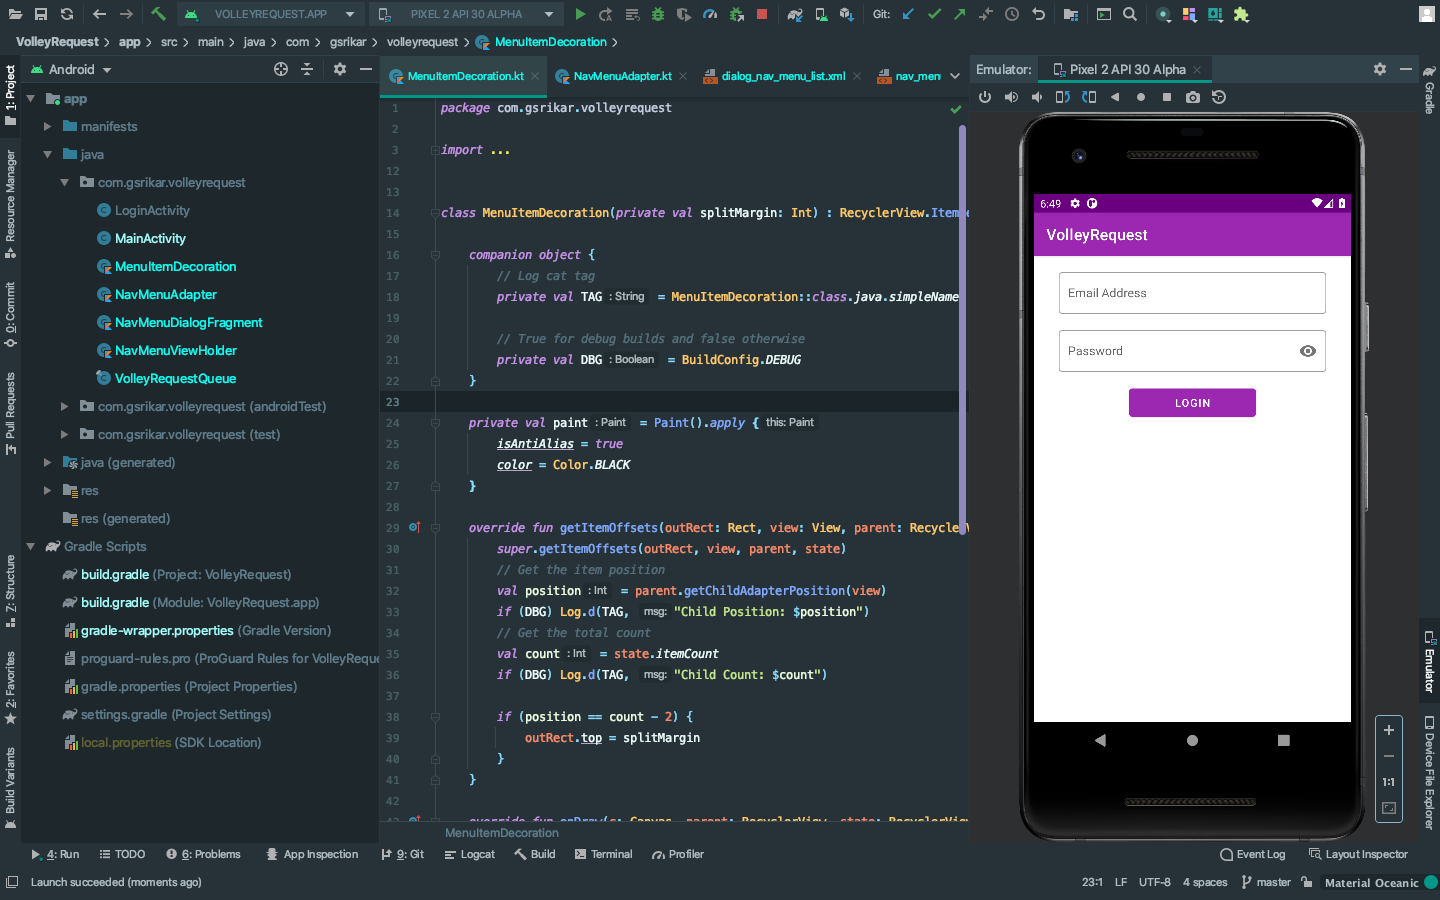
\includegraphics[scale=0.25]{android_studio_emulator.png}
    \caption{Android Studio emulator}
    \label{fig:emulator_android_studija}
\end{figure}
\pagebreak

Alat AVD Menadžer (eng. Android virtual device - AVD) je uključen u Android Studio i u osnovi je emulator koji omogućava pokretanje Android aplikacija na računaru. Zbog toga je vrlo koristan alat jer omogućava brzo testiranje aplikacija bez potrebe za instaliranjem na fizičke uređaje. Pored toga, omogućava simulaciju različitih veličina ekrana, specifikacija, verzija Androida i drugo. Ove pogodnosti dodatno omogućavaju optimizaciju aplikacije za njeno izvršavanje na bilo kojem uređaju.

Android Debug Bridge (ADB) je još jedan od korisnih alata Android Studio-a. U suštini, ovaj alat omogućava terminalni interfejs za interakciju sa telefonom. Kako je Android platforma bazirana na Linuxu, terminalni pristup je jedini način dobijanja admin pristupa. ADB omogućuje most između uređaja i kompjutera.
\pagebreak

\section{Unity 3D}

Unity 3D je višeplatformsko okruženje za razvoj igara sa ugrađenim IDE softverska aplikacija koja pruža pogodnosti programerima pri razvoju softvera. IDE se sastoji od uređivača koda, ispravljača grešaka i takođe poseduje algoritme automatizacije koda, što znatno olakšava rad programerima. \cite{Unity1}

Iako je prva verzija Unity-a, predstavljena na Apple konferenciji “Worldwide Developers Conference” 2005. godine, prvobitno bila namenjena da funkcioniše na Mac računarima, vremenom se razvila i postala dostupna za sve platforme. U narednoj tabeli prikazane su samo neke od važnijih Unity verzija sa novinama koje su za konkretnu verziju karakteristične.

\begin{table}[ht!]
\label{tab:unity_verzije}
\begin{tabular}{|l|l|}
\hline
\multicolumn{1}{|c|}{\textbf{Unity 2.0 (2007)}} & Olakšan rad više programera na istom projektu.\\ \hline
\textbf{Unity 3.0 (2010)}                       & Poboljšane grafičke perfomanse za Desktop računare.                               \\ \hline
\textbf{Unity 4.0 (2012)}                       & Podrška za Adobe Flash, saradnja sa Facebook-om. \\ \hline
\textbf{Unity 2017}                             & Poboljšan rad sa animacijama i kamerama. \\ \hline
\end{tabular}
\end{table}
Unity razvojno okruženje koristi jezik C kao primarni programski jezik.
Kako je poznavanje jezika C i njegovih funkcionalnosti osnova programiranja i kako većina programera jako dobro poznaje ovaj jezik, sa lakoćom se može naviknuti na rad u Unity-ju. Takođe, jezik C ima veoma veliku zajednicu, pa se može očekivati da je problem sa kojim se korisnik sreće već obrađen negde u okviru ove zajednice. Samim tim, programer ima veliku podršku i literaturu koja mu je dostupna pri razvoju softvera u ovom okruženju. Učenje programiranja se zasniva na poznavanju koncepata ovog jezika, svaki početnik će vrlo lako savladati principe Unity okruženja. 

Unity 3D ima široku primenu na velikom broju platformi.
Koju god platformu preferirali, velike su šanse da je Unity podržava.
Slika ispod predstavlja neke od mnogih platforma koje su kompatibilne sa Unity-em (slika \ref{fig:dostupne_platforme}). 

\begin{figure}[ht!]
    \centering
    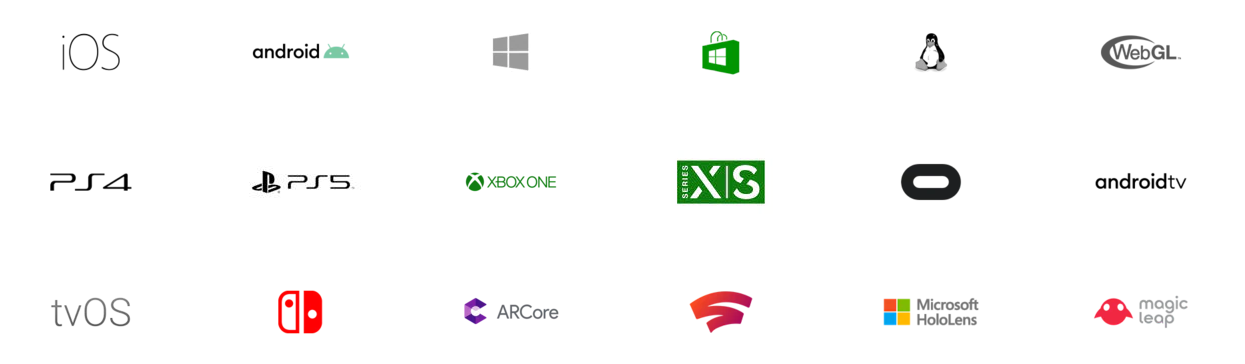
\includegraphics[scale=0.29]{platforme.png}
    \caption{Dostupne platforme}
    \label{fig:dostupne_platforme}
\end{figure}


Unity podržava i dvodimenzionalno (2D) i trodimenzionalno (3D) programiranje. Većina programa u ovakvim situacijama favorizuje jednu opciju i naklonjena je vise ka jednoj od njih, ali to nije slučaj sa Unity razvojnim okruzenjem. Postoji mnoštvo alata, skraćenica i opcija koje omogućavaju olakšan rad početnicima, ali i onima sa više iskustva. 

Interfejs Unity okruženja je jednostavan i intuitivan. 
Ovaj interfejs svakako spada u grupu onih koji su najlakši za korišćenje i usavršavanje. Preglednost i jednostavnost jako su bitne karakteristike
ovog okruženja. Takođe, programeri su u mogućnosti da izgled interfejsa i njegove pogodnosti prilagode sebi i svojim navikama jer je Unity interfejs
podložan modifikacijama. 

Unity u okviru svog okruženja sadrži i \textbf{Asset Store} – platforma na kojoj programeri mogu deliti svoje kodove i biblioteke. Mnoge funkcionalnosti su dostupne potpuno besplatno, takođe, programeri svoje kodove mogu i prodavati u okviru ove platforme. Početnici mogu koristiti ovu prodavnicu i bilbioteke ugrađene u njoj da razviju svoj softver od nule što omogućava lakše upoznavanje sa konceptima programiranja u Unity okruženju.
Sa druge strane, iskusniji programeri neće morati da razvijaju delove softvera koji već postoje, pa tako mogu usmeriti svoje vreme na kreiranje novog softvera.

Unity ima još jednu pogodnost za nove korisnike - potpuno besplatne obuke na svom oficijalnom sajtu.
Bilo da se radi o apsolutnim početnicima ili ipak iskusnijim programerima, ove obuke svima znače jer ih uvode u temu i upoznaju sa mnogim funkcionalnostima ovog razvojnog okruženja.
Sve neophodne dokumentacije i interfejsi su takođe besplatni i dostupni na internetu.

\section{Appcelerator}
Appcelerator je razvojni program za više platforme, kompatibilan za Windows, Android i iOS koji se definiše kao  ''sve što nam je potrebno za kreiranje odličnih, izvornih aplikacija za mobilne uređaje - sve iz jedne osnove JavaScript koda''.\cite{Appcelerator}

Dizajner aplikacija uključuje drag-and-drop za jednostavno postavljanje objekata, a uključena Hyperloop funkcija nam omogućava da koristimo JavaScript da bismo dobili direktan pristup izvornim API-jevima u iOS-u i Android-u.

Još jedna standardna funkcija sa ovim razvojnim programom za razvoj različitih aplikacija je analitika u realnom vremenu koja nam pruža mogućnost da pronađemo i rešavamo probleme sa aplikacijom.

Platforma za razvoj \textit{Titanium}(slika 4), iz Appcelerator-a, pomaže razvoju izvornih mobilnih, tabličnih i desktop aplikacija putem veb programskih jezika kao što su HTML, PHP, JavaScript, Ruby i Python. Ima više od 75.000 mobilnih aplikacija i omogućava korisnicima jednostavan pristup preko 5.000 API-ova i informacija o lokaciji

\begin{figure}[ht!]
    \centering
    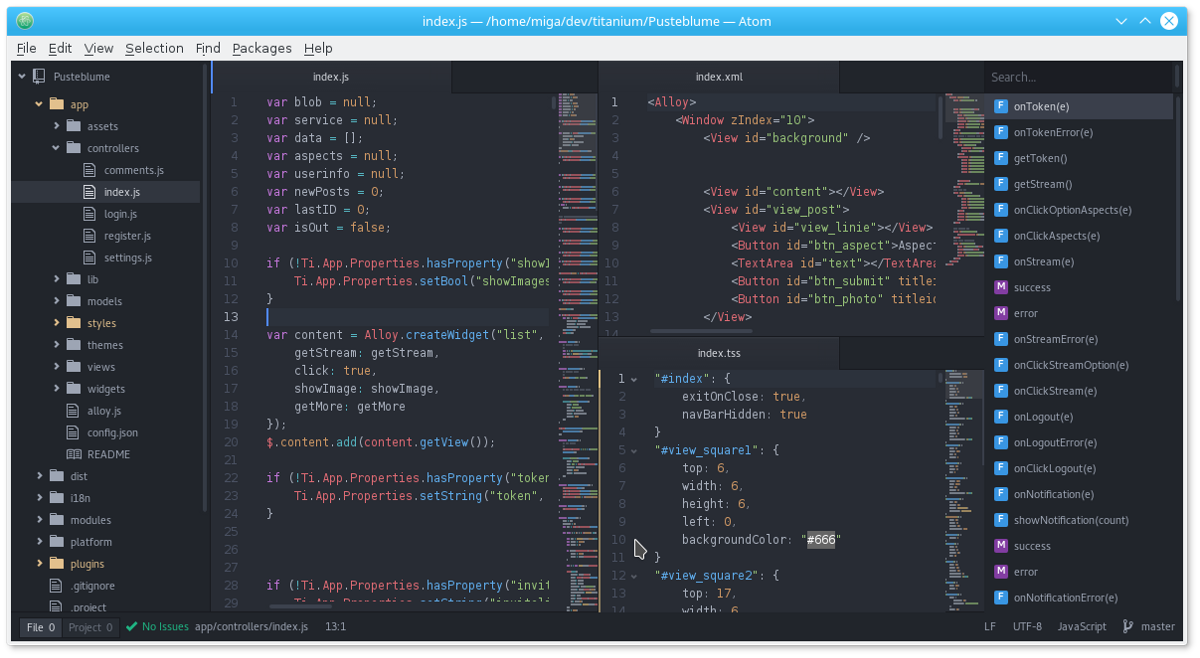
\includegraphics[scale=0.3]{Appcelerator.png}
    \caption{Titanium - primer koda}
\end{figure}

\section{Basic4Android}
Basic4Android, poznatiji kao B4A, je alatka za brzi razvoj aplikacija na Androidu. B4A koriste na desetine hiljada programera iz celog sveta, uključujući i najveće svetske kompanije kao što su NASA, IBM, HP.
B4A i B4i mogu lako isprogramirati aplikacije i za iOS i za Android istovremeno. B4A je alternativa programiranju u Javi. Programski jezik je sličan Visual Basic-u i Visual Basic.Net-u iako je adaptiran prirodnom Android okruženju.

B4A sadrži vizuelni dizajn koji u mnogome olakšava proces pravljenja korisničkog interfejsa, koji se koriste na telefonima i tabletima u različitim veličinama. Kompajlirani programi mogu se testirati u AVD Menadžer emulatorima, ili na pravim Android uređajima koristeći Android Debug Bridge i B4A Bridge. 
B4A generiše standardne Android aplikacije koje mogu biti postavljene na prodavnicama aplikacija poput Google Play-a, Samsung Apps-a, Amazon Appstore-a.

B4A podržava sve tipove aplikacija kao što su igrice, baze podataka. Primer koda u B4A se može videti ispod
\begin{figure}[ht!]
    \centering
    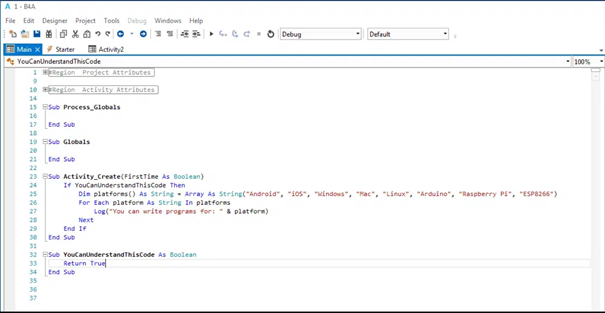
\includegraphics[scale=0.9]{b4aslika.png}
    \caption{Primer koda u B4A}
\end{figure}
\section{Zaključak}

Android je projekat koji mnogo obećava. Jedna od njegovih glavnih prednosti je dobra organizacija,
koja ima potencijal da iskoristi svu moć i znanje zajednice otvorenog koda.
Još jedna dobra stvar je uključenost velikog broja jakih kompanija u projekat, što omogućuje jako brzo širenje.
Brži razvoj, kao posledica dobre organizacije, povlači za sobom unapredivanje svih aspekata projekta.
Svako može učestvovati, što će dodatno podsticati inovacije i ubrzati razvoj. 
Svakodnevno se platforma tehnički usavršava i unapreduje od strane nezavisnih proizvodača. 
Android je vodeći operativni sistem za mobilne telefone i pretpostavlja se da će i u budućnosti biti u vrhu i doneti
mnoštvo inovacija. Zbog svega navedenog, okruženja koja nam pomažu prilikom
razvoja aplikacja za Android igraju veoma značajnu ulogu u svetu Andorid programiranja.
\\\\\\\\\\

\begin{thebibliography}{}
\bibitem{Unity1}Unity 3D - https://www.mindinventory.com/blog/unity-3d-game-development/
\bibitem{Appcelerator}Appcelerator - https://bs.eyewated.com/top-5-alatki-za-razvoj-multiformnih-mobilnih-aplikacija/
\bibitem{Alati2}Alati za programere - https://www.androidsis.com/bs/najbolji-alati-za-programere-android-aplikacija/
\bibitem{Android Studio}Android Studio - https://androidayuda.com/bs/android-studio/
\end{thebibliography}

\end{document}
